\documentclass[11pt,a4paper]{article}
\usepackage[utf8]{inputenc}
\usepackage[spanish]{babel}
\usepackage{geometry}
\geometry{left=2.5cm,right=2.5cm,top=2.5cm,bottom=2.5cm}
\usepackage{booktabs}
\usepackage{amsmath}
\usepackage{tabularx}
\usepackage{graphicx} % Paquete fundamental para insertar las graficas
\usepackage{float}    % Para forzar la posicion de las imagenes
\usepackage{hyperref}

\title{\textbf{Proyecto de Computación de Alto Rendimiento (HPC): \\ Paralelización de la Ecuación de Poisson en 2D con OpenMP}}
\author{
    \begin{tabular}{c}
    Camilo Huertas \quad Sebastián Rodriguez \\
    \textit{Programa Académico de Física} \\
    \textit{Universidad Distrital Francisco José de Caldas} \\
    \end{tabular}
}
\date{24 de marzo de 2026}

\begin{document}

\maketitle

\section*{Objetivo}
Aplicar diferentes directivas de OpenMP para paralelizar un código secuencial que resuelve la ecuación de Poisson 2D mediante diferencias finitas. Se realizará un barrido paramétrico masivo variando la densidad de la grilla espacial y el número de hilos de procesamiento para evaluar la escalabilidad, los cuellos de botella de memoria y el límite de aceleración (Ley de Amdahl).

\section*{Especificaciones del Sistema y Metodología}
Todas las pruebas de rendimiento registradas en este informe fueron ejecutadas en un servidor HPC con la siguiente configuración:
\begin{itemize}
    \item \textbf{Procesador:} AMD Ryzen Threadripper 3990X 64-Core Processor.
    \item \textbf{Arquitectura:} x86\_64.
    \item \textbf{Caché L3:} 256 MiB.
    \item \textbf{Núcleos físicos:} 64.
    \item \textbf{Hilos lógicos (\textit{Threads}):} 128.
\end{itemize}

\textit{Nota metodológica:} En lugar de realizar una prueba estática, se programó un entorno de automatización (Makefile + script en C++) para realizar un barrido variando las mallas espaciales ($M \times N$) en tamaños de $50\times50$, $100\times100$ y $200\times200$. Para cada escenario se forzó explícitamente el uso de 1, 2, 4, 8, 16, 32, 64 y 80 hilos lógicos mediante \texttt{omp\_set\_num\_threads()}.

\section*{Análisis de Escalabilidad Visual}

En la siguiente figura se exponen las curvas de rendimiento computacional para los tres tamaños de malla. Se observa una escala logarítmica tanto en el número de hilos (eje X) como en el tiempo de ejecución (eje Y).

\begin{figure}[H]
    \centering
    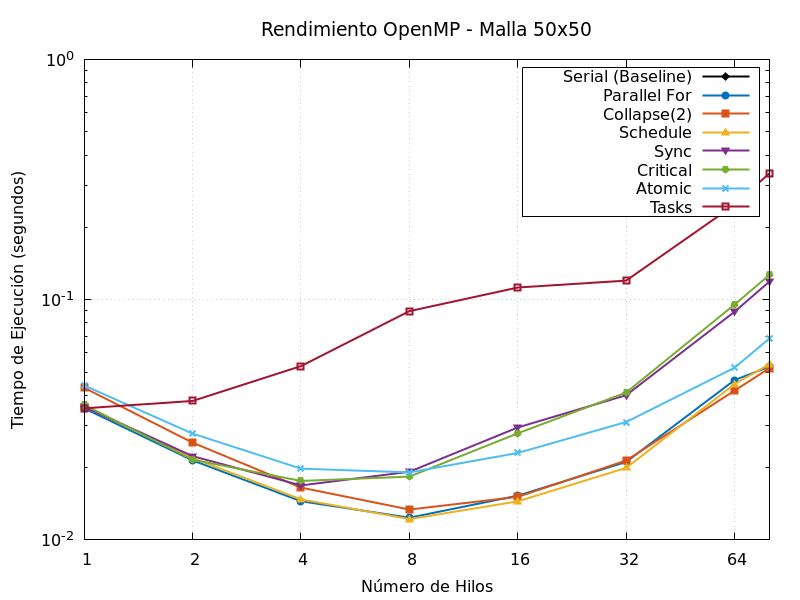
\includegraphics[width=0.48\textwidth]{../imag/comparativa_malla_50.png}
    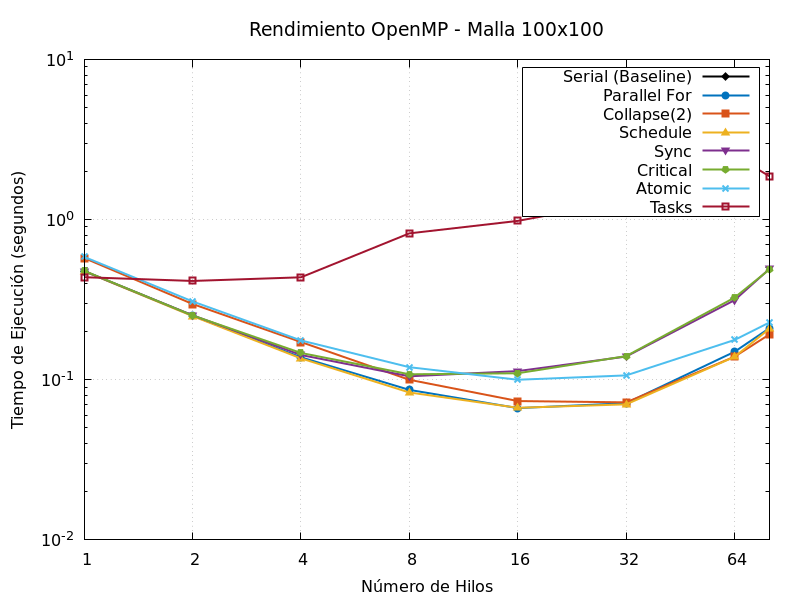
\includegraphics[width=0.48\textwidth]{../imag/comparativa_malla_100.png}
    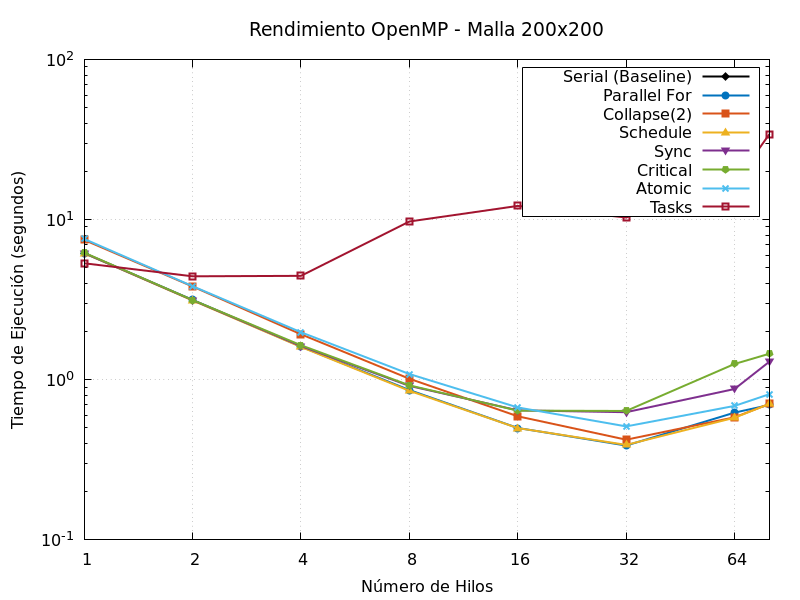
\includegraphics[width=0.8\textwidth]{../imag/comparativa_malla_200.png}
    \caption{Curvas de rendimiento para mallas 50x50, 100x100 y 200x200.}
    \label{fig:rendimiento}
\end{figure}

Como se evidencia en las gráficas, sin importar el tamaño de la malla, el límite de máxima eficiencia o ``punto dulce'' (\textit{sweet spot}) se alcanza a los \textbf{32 hilos}. A partir de los 64 hilos, las curvas de tiempo sufren una inflexión al alza, demostrando una degradación del rendimiento debido a la saturación del ancho de banda de la memoria compartida (cuello de botella de Von Neumann) y el sobrecosto de sincronización.

\section*{Análisis por Directivas (Basado en Malla $200\times200$)}

Para evitar redundancias, el análisis cuantitativo de las actividades se concentrará en el caso de mayor exigencia computacional (malla $200\times200$), cuyo tiempo secuencial base fue de \textbf{6.185 segundos}.

\subsection*{Actividad 1: \texttt{\#pragma omp parallel for}}
Se paralelizó el bucle principal. 
\begin{itemize}
    \item \textbf{Mejor tiempo (32 hilos):} 0.388 segundos.
    \item \textbf{Análisis:} Presenta la aceleración más estable y eficiente de todo el experimento. Logró un \textit{Speedup} máximo de casi 16x respecto al código secuencial. La inclusión de \texttt{reduction(max:delta)} operó sin ralentizaciones significativas.
\end{itemize}

\subsection*{Actividad 2: \texttt{collapse(2)}}
\begin{itemize}
    \item \textbf{Mejor tiempo (32 hilos):} 0.422 segundos.
    \item \textbf{Análisis:} A pesar de aplanar los bucles $i$ y $j$, introdujo un sobrecosto algebraico en la gestión de índices que lo hizo levemente más lento que el \texttt{parallel for} simple en todos los escenarios.
\end{itemize}

\subsection*{Actividades 4 y 5: \texttt{schedule} y Control de Sincronización (\texttt{critical})}
\begin{itemize}
    \item \textbf{Mejor tiempo \texttt{schedule} (32 hilos):} 0.391 segundos.
    \item \textbf{Mejor tiempo \texttt{critical} (32 hilos):} 0.638 segundos.
    \item \textbf{Análisis:} El control mediante \texttt{schedule(static)} mantuvo un rendimiento idéntico a la Actividad 1. Por otro lado, la sincronización manual explícita y el uso de regiones \texttt{critical} afectaron la fluidez de la concurrencia, elevando el tiempo óptimo en más de un 60\% respecto al código sin barreras innecesarias.
\end{itemize}

\subsection*{Actividad 6: Variables Compartidas (\texttt{atomic} vs \texttt{critical})}
\begin{itemize}
    \item \textbf{Mejor tiempo \texttt{atomic} (32 hilos):} 0.511 segundos.
    \item \textbf{Análisis:} En operaciones matemáticas de un solo ciclo (como el incremento de un contador), la instrucción atómica a nivel de hardware superó sustancialmente a la región \texttt{critical} (0.511s frente a 0.638s), confirmando su menor latencia y \textit{overhead}.
\end{itemize}

\subsection*{Actividad 7: Exploración con Tareas (\texttt{task})}
\begin{itemize}
    \item \textbf{Tiempo mínimo (2 hilos):} 4.43 segundos.
    \item \textbf{Tiempo máximo (80 hilos):} 34.28 segundos.
    \item \textbf{Análisis:} Fue la peor directiva evaluada con diferencia. Como se observa en la curva roja oscura de la gráfica, escalar esta directiva resulta contraproducente. La sobrecarga administrativa (crear, poner en cola y despachar decenas de miles de tareas para bloques regulares) estranguló al despachador de OpenMP, siendo hasta 5 veces más lento que correr el código secuencial puro.
\end{itemize}

\section*{Comparación Final de Estrategias}

\begin{table}[H]
\centering
\begin{tabularx}{\textwidth}{llccl}
\toprule
\textbf{Versión} & \textbf{Directiva} & \textbf{Mejor Tiempo} & \textbf{Hilos Óptimos} & \textbf{Eficiencia HPC} \\
\midrule
Secuencial & N/A & 6.185 s & 1 & Línea base (Referencia) \\
Parallel For & \texttt{parallel for} & \textbf{0.388 s} & \textbf{32} & \textbf{Rendimiento Superior} \\
Schedule & \texttt{schedule} & 0.391 s & 32 & Equivalente al básico \\
Collapse & \texttt{collapse(2)} & 0.422 s & 32 & Penalización leve de overhead \\
Atomic & \texttt{atomic} & 0.511 s & 32 & Menor impacto que critical \\
Critical & \texttt{critical} & 0.638 s & 32 & Cuello de botella en sincronización\\
Tareas & \texttt{task} & 4.430 s & 2 & Sobrecarga catastrófica \\
\bottomrule
\end{tabularx}
\caption{Comparativa de tiempos óptimos en la Malla 200x200.}
\end{table}

\section*{Conclusiones Generales}
\begin{enumerate}
    \item \textbf{¿Cuál fue la versión más rápida y la más eficiente?} \\
    La directiva \texttt{\#pragma omp parallel for} con una planificación básica. Además, se comprobó que el máximo rendimiento se alcanza a los \textbf{32 hilos}, superando ese umbral el paralelismo se vuelve contraproducente por el costo de comunicación y transferencia a caché.
    \item \textbf{¿Qué directiva es más fácil de usar y robusta?} \\
    Nuevamente \texttt{parallel for} con la cláusula \texttt{reduction}. Proporciona el máximo rendimiento con la menor cantidad de intervención en el código base.
    \item \textbf{¿Hubo directivas que empeoraron el rendimiento?} \\
    De forma contundente, la directiva \texttt{task}. Para la resolución de ecuaciones diferenciales en grillas matriciales uniformes y densas, el modelo de bucles (\texttt{for}) es superior. Las tareas (\texttt{task}) solo deben usarse para flujos de control asimétricos o estructuras irregulares (árboles, listas recursivas).
\end{enumerate}

\end{document}
